% 第 10 章 Using the Error Browser
\bichapter{使用错误浏览器}{Using the Error Browser}
\label{chap:gui-error}

IC Compiler II GUI 提供错误浏览器（error browser）工具，用于查看错误消息和信息性消息（informational message），在版图视图（layout view）中高亮相关对象，并处置（disposition）错误。使用错误浏览器可以快速选出一组待复查的错误，定位某一条特定错误，并在版图中调查该问题。

本章包括以下主题：
\begin{itemize}
  \item 错误浏览器概述
  \item 加载与保存错误数据
  \item 管理错误层次
  \item 管理错误列表并查看错误详情
  \item 使用错误过滤器
  \item 高亮错误
  \item 将错误标记为已修复并更改错误状态
  \item 写出设计规则检查（DRC）错误数据
\end{itemize}

\section{错误浏览器概述}
\subsection*{Error Browser Overview}

错误浏览器提供若干功能，帮助复查错误、处置错误，并把更新后的错误文件保存到磁盘。在错误浏览器中选中错误时，版图查看器（layout viewer）会平移到错误所在位置并放大，以便在视图中单独观察该错误。

\begin{noteBox}
错误浏览器缩放或平移以显示所选错误时，只有活动版图视图会随之改变。
\end{noteBox}

错误浏览器按错误类型（error type）把错误归组。错误类型由生成该错误的 GUI 任务或 Tcl 命令指定。每条错误包含简短描述、该错误的包围盒（bounding box）坐标，以及关于该错误的其他信息。

要启动错误浏览器，选择 \textbf{View > Error Browser}。第一次打开错误浏览器时，工具会显示一个对话框，其中列出可用的错误消息文件、生成该文件的检查任务（checking task），以及文件上次被修改的时间。在列表中选择一项，然后单击 Open Selected 继续。错误浏览器见图~\ref{fig:gui-133}。

\begin{figure}[htbp]
\centering
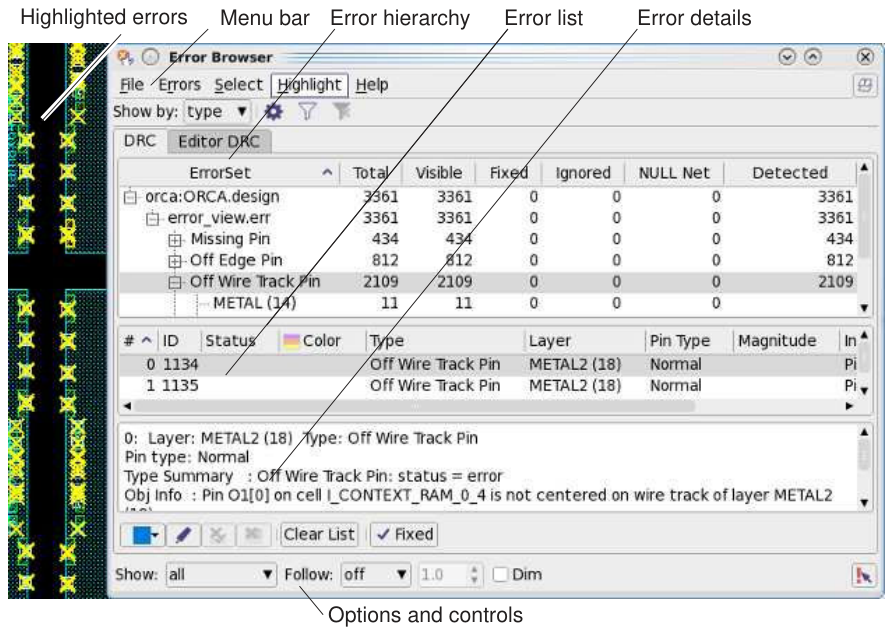
\includegraphics[width=0.92\textwidth]{gui-fig-133.png}
\caption{错误浏览器}
\label{fig:gui-133}
\end{figure}

用错误浏览器调试错误的典型流程包括以下步骤：
\begin{enumerate}
  \item 验证设计并保存结果。
  \item 在错误浏览器中打开已保存的错误文件。
  \item 选择一组要复查的错误。\\
        可以按错误类型分组，也可以按与这些错误关联的层（layer）分组。还可以按错误在设计中的物理位置选择一组错误。
  \item 在列表中选中错误，并在版图视图中查看错误的上下文，从而逐条分析并调试。
  \item 在版图视图中改正错误，并在错误浏览器中把该错误标为已修复（fixed）或已忽略（ignored）。
  \item （可选）隐藏已修复的错误。
\end{enumerate}

\section{加载与保存错误数据}
\subsection*{Loading and Saving Error Data}

默认情况下，错误浏览器读取并写入与当前块（block）关联的错误数据（error data）文件。这些文件使用 \cmd{.err} 扩展名，保存在该块的库目录（library directory）中。也可以保存和加载不与该块关联的 XML 格式错误数据文件。

要打开与当前块关联的已有错误数据文件：
\begin{enumerate}
  \item 选择 \textbf{File > Open}，打开 Open Error Data 对话框。
  \item 选择要打开的错误数据文件。
  \item 单击 Open Selected 按钮。
\end{enumerate}

要打开扩展名为 \cmd{.err} 的错误数据文件，或非托管的 XML 格式错误数据文件：
\begin{enumerate}
  \item 选择 \textbf{File > Read Error File}，打开文件浏览器。
  \item 选择要打开的文件。\\
        若文件扩展名为 \cmd{.xml}，请在 Open Error Data File 对话框的 Files of type 框中选择 Any files。
  \item 单击 OK。
\end{enumerate}

更新已修复状态或做了其他更改之后，要保存对错误数据的更改：
\begin{enumerate}
  \item 选择 \textbf{File > Save}。
  \item 单击 Save 按钮。
\end{enumerate}

工具把错误浏览器的当前状态写入输出文件。若没有打开的错误数据文件，或者错误数据没有更改，该菜单操作处于禁用状态。

要以其他格式保存错误数据：
\begin{itemize}
  \item 选择 \textbf{File > Export as CSV}，把错误数据写成逗号分隔值（comma-separated values，CSV）。
  \item 选择 \textbf{File > Export to Error File}，把这些信息写成错误数据。
\end{itemize}

\section{管理错误层次}
\subsection*{Managing the Error Hierarchy}

错误浏览器在菜单栏下方显示两个选项卡：DRC 与 Editor DRC。DRC 选项卡中的列表显示当前错误数据文件里的错误层次（error hierarchy）。可以对错误层次列表执行下列操作：
\begin{itemize}
  \item 单击 ErrorSet 列左侧的 [+] 按钮展开列表，或单击 [-] 按钮折叠列表。
  \item 单击列标题，对该列排序，或更改该列的排序方向。
  \item 把指针移到列表中的某一行上，在信息提示（infotip）中显示信息。
  \item 单击列表中的某一行，在版图视图中平移并缩放到该错误，并在浏览器的错误列表区域显示更多信息。
  \item 单击某一行，按住 Shift 键，再单击列表中更靠下的另一行，以选中这一范围内的各行。
  \item 单击某一行，按住 Ctrl 键，再单击第二行，以选中多行。继续按住 Ctrl 键并单击其他行，把它们加入选择。
  \item 右键单击鼠标，显示上下文菜单（context menu）；从菜单中选择一项，可以打开新的错误数据、保存当前错误数据、把当前错误标为已修复，以及执行其他同类操作。
  \item 从错误浏览器菜单选择 \textbf{Errors > Next Error Group} 或 \textbf{Errors > Previous Error Group}，转到错误层次中的另一个错误组。
\end{itemize}

\section{管理错误列表并查看错误详情}
\subsection*{Managing the Error List and Viewing Error Details}

在错误层次列表下方，工具显示错误列表（error list）。错误列表列出你在工具的错误层次区域中所选错误类型下的各条错误。可以对错误列表执行下列操作：
\begin{itemize}
  \item 单击列标题，对该列排序，或更改该列的排序方向。
  \item 单击并拖动列标题，以调整各列的顺序。
  \item 把指针移到列表中的某一行上，在信息提示中显示信息。
  \item 单击列表中的某一行，在版图视图中平移并缩放到该错误，并在浏览器的错误列表区域显示更多信息。
  \item 右键单击鼠标，显示上下文菜单；从菜单中选择一项，可以切换该错误的已修复状态、高亮错误，以及执行其他同类操作。
  \item 按住 Ctrl 或 Shift 键并单击列表中的其他行，或沿列表向下单击并拖动鼠标，以选择多条错误。
  \item 选择上下文菜单中的相应项，或选择 \textbf{Errors > Clear Error List}，清空该列表。
  \item 从错误浏览器菜单选择 \textbf{Errors > Next Error Group} 或 \textbf{Errors > Previous Error Group}，转到错误列表中的另一组。
\end{itemize}

错误浏览器在错误列表下方的错误详情（error detail）区域显示所选错误的详情。把指针停在错误详情窗格上，会显示包含错误详情的信息提示。

\section{使用错误过滤器}
\subsection*{Using Error Filters}

使用错误过滤，可以暂时把错误从错误浏览器和版图视图中去掉。通过 Set Error Data Filter 对话框应用过滤器（filter），见图~\ref{fig:gui-134}。

要创建错误过滤器：
\begin{enumerate}
  \item 选择 \textbf{Errors > Set Filter}。
  \item 选择 Show only matching errors 或 Hide matching errors，以设置过滤器类型。
  \item 选择错误类型、层设置、线网（net）以及其他设置，从而建立过滤条件。
  \item 单击 Apply 或 OK 以应用过滤器，或单击 Clear Filter 以去掉过滤器。
\end{enumerate}

创建过滤器之后，该过滤器会作用于当前已经打开的错误数据，以及在当前会话中打开的任何其他错误数据。过滤器不会累积；应用新的过滤器会覆盖此前设置的任何过滤器。要清除过滤器，选择 \textbf{Errors > Clear Filter}，或在 Set Error Data Filter 对话框中单击 Clear Filter。

\begin{figure}[htbp]
\centering
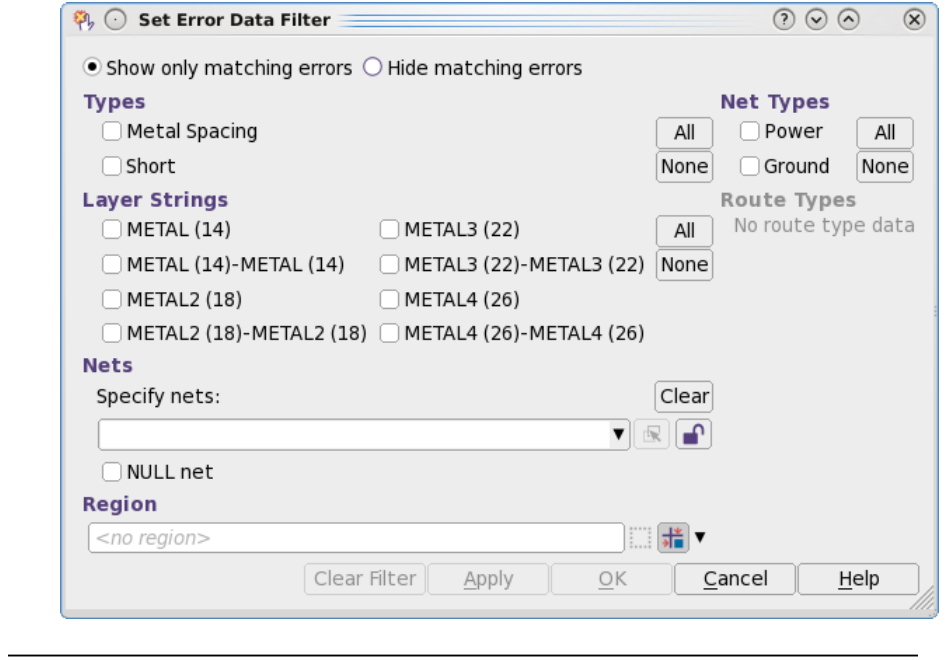
\includegraphics[width=0.92\textwidth]{gui-fig-134.png}
\caption{Set Error Data Filter 对话框}
\label{fig:gui-134}
\end{figure}

\section{高亮错误}
\subsection*{Highlighting Errors}

可以给版图视图中的错误加上不同的高亮（highlight）颜色。使用 Highlight 菜单来高亮错误，或去掉高亮。也可以使用 GUI 底部的高亮按钮完成这些操作。Highlight 菜单提供下列菜单命令：
\begin{itemize}
  \item By Type, Layer, Net：打开 Highlight Errors 对话框，按错误类型、层字符串（layer string）或关联线网高亮错误。
  \item Selected：用当前高亮颜色高亮所选错误。
  \item All Errors in List：用当前高亮颜色高亮错误列表中的全部可见错误。
  \item Clear Selected：清除所选错误上的高亮颜色。
  \item Clear Current Color：清除当前高亮颜色的全部高亮。
  \item Clear All：清除全部错误高亮。
  \item Set Current Color：提供颜色菜单，用来选定当前高亮颜色。
  \item Next Color：把当前高亮颜色切换为 Set Current Color 菜单中的下一种颜色。
  \item Auto Cycle Colors：切换此选项。启用后，每执行一次 \textbf{Highlight > Selected}，当前高亮颜色就改为下一种颜色。
  \item Error Highlight Counts：打开一个对话框，显示每个高亮集合中的错误数量，以及一张简单直方图（histogram）。
\end{itemize}

\section{将错误标记为已修复并更改错误状态}
\subsection*{Marking Errors as Fixed and Changing Error Status}

要更改某条错误的状态，先在错误列表中选择一条或多条错误，然后执行下列操作之一：
\begin{itemize}
  \item 单击 Fixed 按钮，切换 Status 列中的已修复状态值。
  \item 单击鼠标右键并选择 Set Status，然后按需要选择 Error、Fixed 或 Ignored。也可以从错误浏览器菜单选择 \textbf{Errors > Set Status}，并做相同的选择。
\end{itemize}

这些操作会更改所选错误的状态。Status 列中的值变为对勾，表示该错误已修复；该标记被清除，表示错误尚未修复；变为 (X)，表示处于已忽略状态。

\section{写出设计规则检查（DRC）错误数据}
\subsection*{Writing Out DRC Error Data}

错误浏览器提供图形工具，用来复查工具中各条检查命令所报告的错误。要把某个错误数据文件中的错误写成文本报告，使用 \cmd{report\_drc\_errors} 命令，并用选项报告特定的错误类型，或报告特定层上的错误。

该命令可以写出下列类型的报告：\cmd{error\_type}、\cmd{error\_layer}、\cmd{detailed} 和 \cmd{matrix}。使用 \opt{-report\_type} 选项指定报告类型。\cmd{error\_type} 报告是默认报告类型，不指定选项时就会生成，也可以通过指定 \opt{-report\_type error\_type} 生成。它列出每种错误类型及其计数，如下例所示。\cmd{error\_layer} 报告由 \opt{-report\_type error\_layer} 选项生成，与 \cmd{error\_type} 报告类似，但先按层分组，再按错误类型分组。

\begin{lstlisting}
ErrorSet                                 Total  Visible  Fixed  Ignored
-----------------------------------------------------------------------
Design : test                            54     3        0      0
      Data : zroute.err                  54     3        0      0
            Net                          3      1        0      0
                METAL3 (28)              1      1        0      0
            Route Spacing                6      2        0      0
                METAL2 (18)-METAL3 (28)  1      1        0      0
                METAL3 (28)-METAL4 (31)  1      1        0      0
\end{lstlisting}

\cmd{detailed} 报告由 \opt{-report\_type detailed} 选项生成。它为每条错误报告错误标识（error ID）、错误类型以及其他信息，内容与错误浏览器中显示的完整错误信息类似。详细报告如下例所示。

\begin{lstlisting}
Error ID          : 1
Error Type        : Route Spacing
Error Layer       : METAL3 (28)-METAL4 (31)
Number of errors  : 6
Description       : Spacing violation between
                    hmg_out44_10_ and RES_I109_X9
                    on layers {METAL3 (28) METAL4 (31)} --
                    direction: vertical, required: 1.2 um, actual: 0.6 um
Status            : error
Bbox              : {293.8000 364.4000} {294.2000 366.8000}

Error ID          : 3
Error Type        : Route Spacing
Error Layer       : METAL2 (18)-METAL3 (28)
Number of errors  : 6
Description       : Spacing violation between A0_9_ and
                    B0_9_ on layers {METAL2 (18) METAL3 (28)} --
                    direction: upper left to lower right, required:
                    1.2000 um, actual: 0.6000 um
Status            : error
Bbox              : {261.0000 301.8000} {261.4000 303.0000}
\end{lstlisting}

下列示例按所用的命令选项写出不同的错误报告：
\begin{itemize}
  \item 为错误数据文件中的全部错误写出默认的 \cmd{error\_data} 错误报告。
\end{itemize}
\begin{lstlisting}
icc2_shell> report_drc_errors -error_data zroute.err
\end{lstlisting}
\begin{itemize}
  \item 只为 METAL3 层上、错误类型为 Route Spacing 和 Net 的错误写出详细报告。
\end{itemize}
\begin{lstlisting}
icc2_shell> set type [get_drc_error_types \
   -error_data zroute.err {{Route Spacing} {Net}}]
icc2_shell> report_drc_errors -error_data zroute.err \
   -report_type detailed -error_type $type -layers {METAL3}
\end{lstlisting}
